\chapter{Metodologia}

\section{Bancada experimental}

A bancada experimental consiste em uma unidade laboratorial de dessalinização, comercializada pela empresa Aquastil \cite{Aquastill2025}, adaptada para operar com o módulo fabicado no laboratório de nano e microfluidica e microssistemas (LabMEMS). A unidade possui três reservatórios d'água destinados a água de produção (quente), água para refrigeração (frio) e permeado. O aquecimento da água de produção é realizado por um sistema on/off através do controlador MT-516E da FULLGAUGE e uma resistência de 2~kW posicionada no interior do reservatório. O resfriamento da água de refrigeração é realizado através de um sistema HVAC (heating, ventilation and air contitioning). A figura \ref{fig:bancada} apresenta a bancada vista de frente.


\begin{figure}[H]
    \centering
    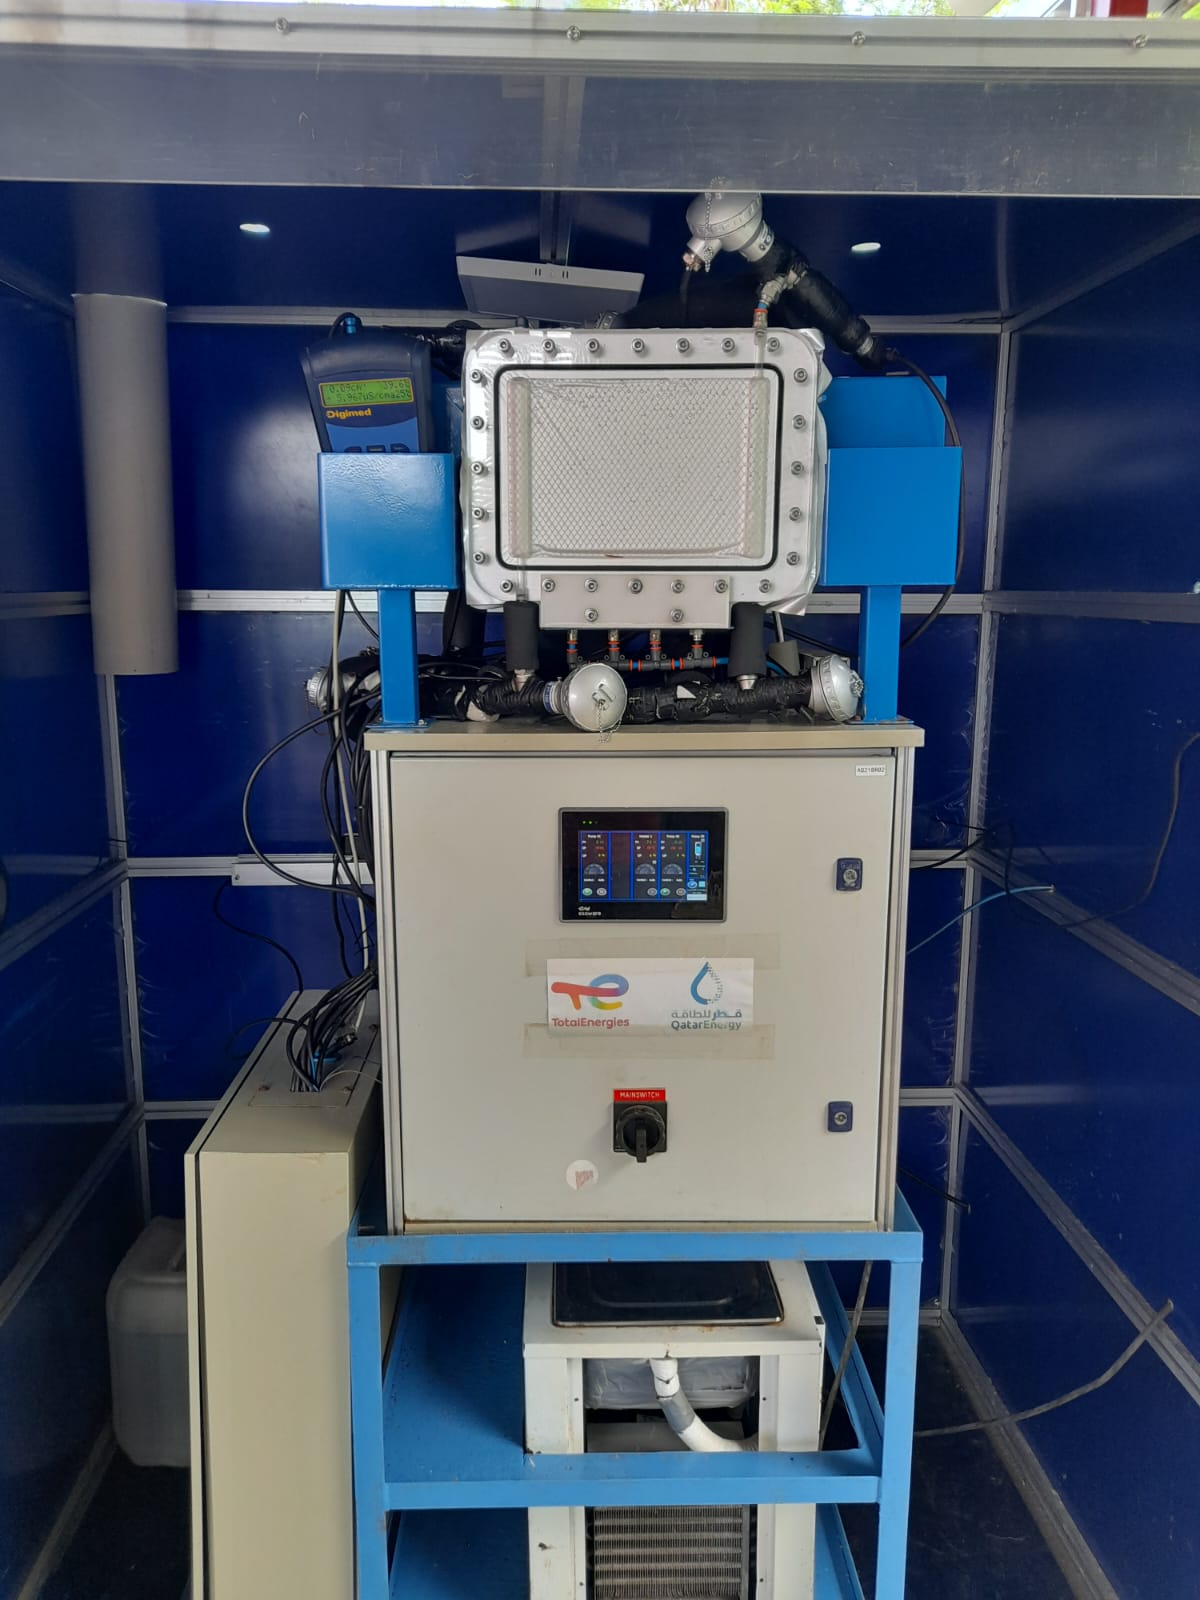
\includegraphics[width=\textwidth, height=9cm, keepaspectratio]{bancada.jpeg}
    \caption{Bancada utilizada para a realização dos experimentos.}
    \label{fig:bancada}
\end{figure}

A bancada também possui três bombas, uma para cada reservatório, as quais fornecem a alimentação do módulo AGMD, e uma para retornar o permeado produzido de volta ao reservatório de água de produção. A bancada é equipada com sensores de temperatura e pressão nas entradas e saídas do módulo, assim como sensores de vazão após as bombas dos reservatórios quente e frio. Há também uma célula de condutividade posicionada na linha de entrada do tanque de permeado. A tabela \ref{tab:sensores} apresenta as caracteristicas dos sensores utilizados e a figura \ref{fig:diagramabancada} o diagrama da bancada.

\begin{table}[H]
\centering
\caption{Sensores utilizados na bancada experimental.}
\label{tab:sensores}
\resizebox{\textwidth}{!}{%
\begin{tabular}{lllll}
\hline
\textbf{Sensor} & \textbf{Variável} & \textbf{Fabricante} & \textbf{Intervalo} & \textbf{Incerteza} \\ \hline
PT100 & Temperatura & Omega \cite{Omega} & 0--100~$^\circ$C & $\pm0.5~^\circ$C \\
Condutivímetro & Condutividade & Digimed \cite{Digimed} & 0--500~$mScm^{-1}$ & $\pm1\%$ da leitura \\
Transmissor de pressão & Pressão & Burkert \cite{Burkert1} & 0--10~bar & $\pm0,5\%$ FS \\
Medidor de vazão & Vazão & Burkert \cite{Burkert2} & 0,1--10~$Lmin^{-1}$ & $\pm1,5\%$ da leitura \\
\hline
\end{tabular}%
}
\end{table}

\begin{figure}[H]
    \centering
    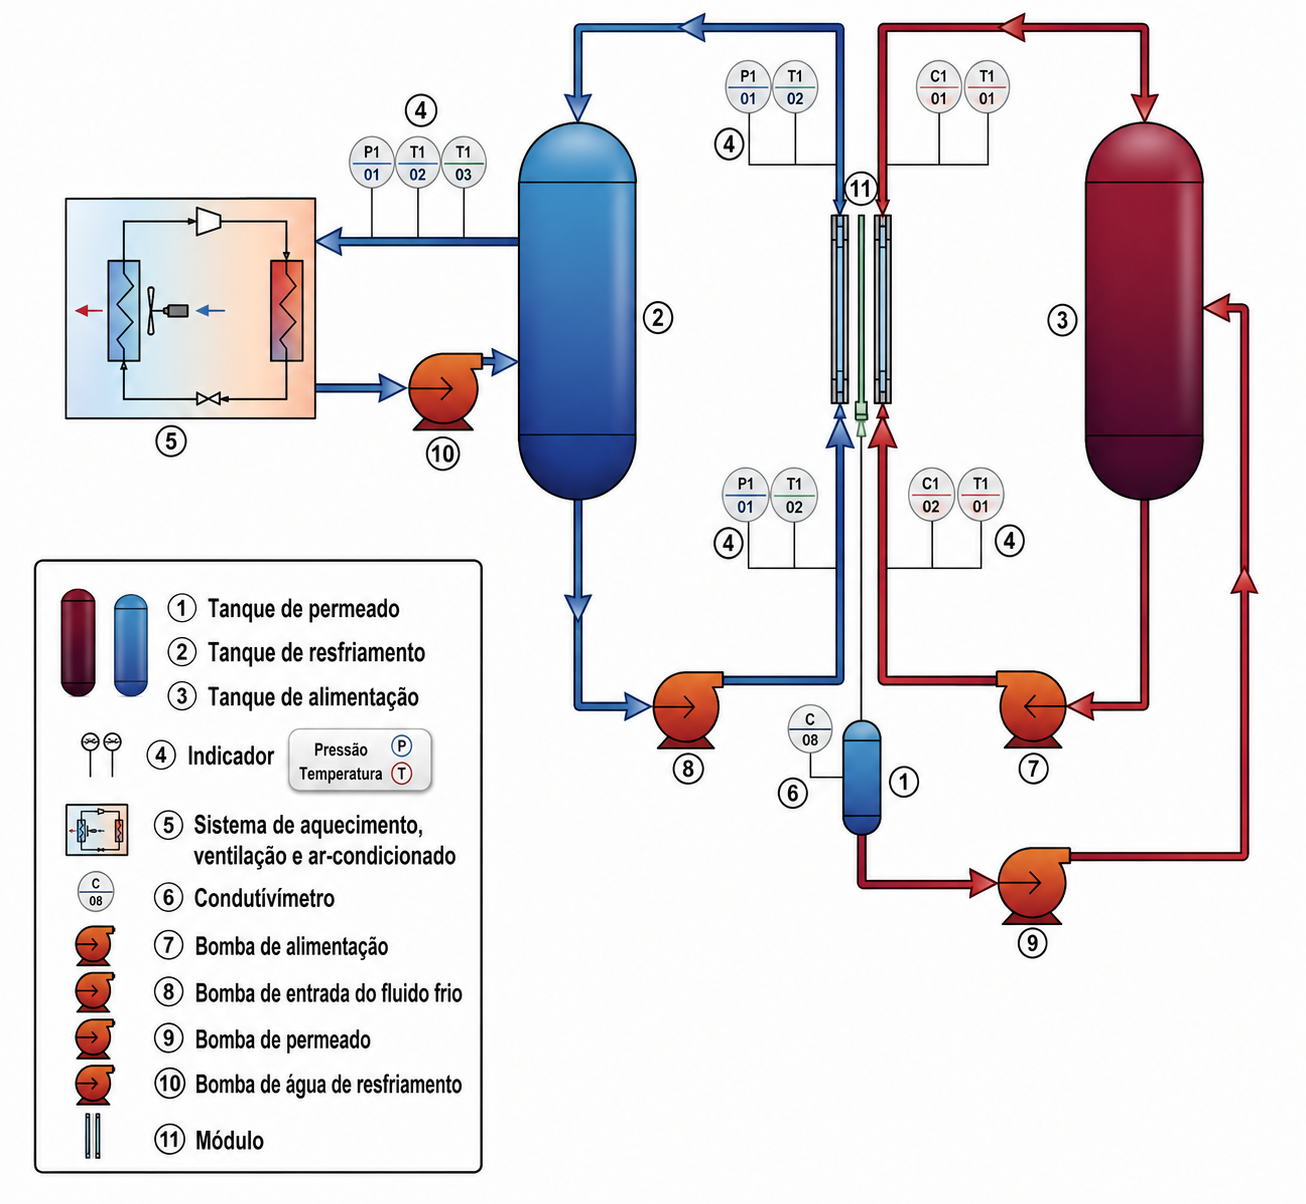
\includegraphics[width=\textwidth, height=12cm, keepaspectratio]{diagramabancada.png}
    \caption{Diagrama da bancada experimental de destilação por membranas com gap de ar (AGMD), contendo os tanques de alimentação, resfriamento e permeado, módulo de membrana, sistema HVAC, bombas de circulação e instrumentos de monitoramento de pressão, temperatura e condutividade.}
    \label{fig:diagramabancada}
\end{figure}

Os principais componentes do módulo AGMD são duas faces externas fabricadas em acrílico, uma folha de alumínio, um espaçador e a membrana a ser testada, a figura \ref{fig:vistaexplodida} apresenta uma vista expodida com estes componentes, enquanto a figura \ref{fig:modulomontado} apresenta o módulo montado.



\begin{figure}[H]
    \centering
    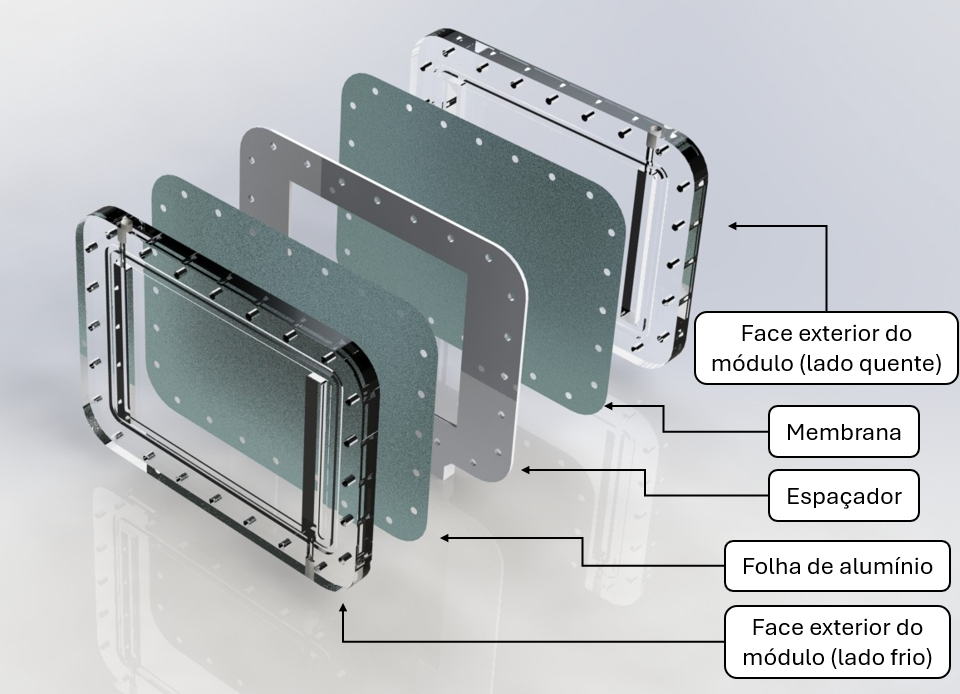
\includegraphics[width=\textwidth, height=7cm, keepaspectratio]{vistaexplodida.png}
    \caption{Vista explodida do módulo AGMD representado seus principais componentes.}
    \label{fig:vistaexplodida}
\end{figure}

\begin{figure}[H]
    \centering
    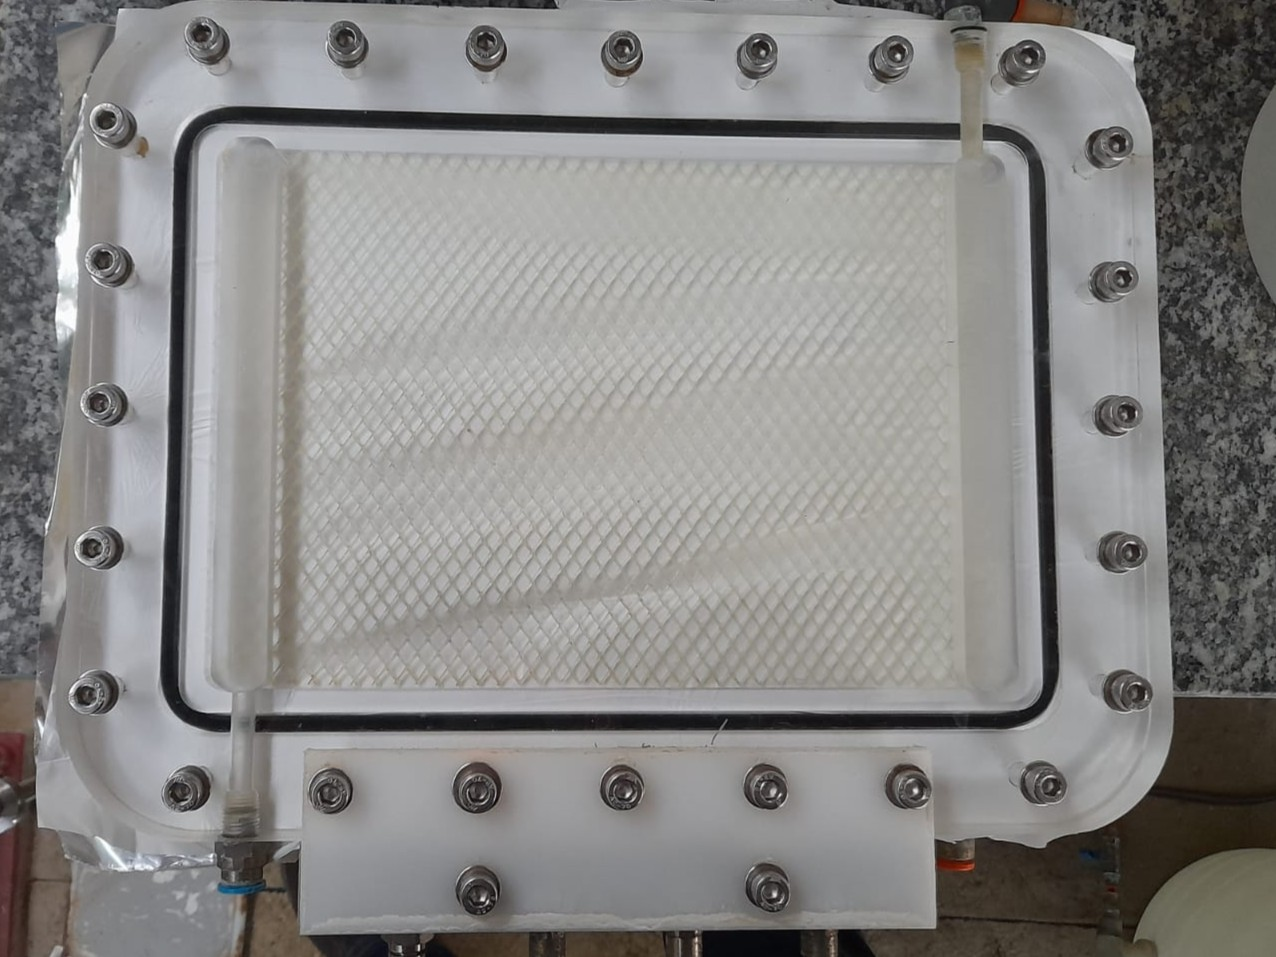
\includegraphics[width=\textwidth, height=7cm, keepaspectratio]{modulomontado.jpeg}
    \caption{Módulo montado em bancada.}
    \label{fig:modulomontado}
\end{figure}

Os experimentos serão realizados adotando a temperatura do lado quente em 70~$^\circ$C e do lado frio em 25~$^\circ$C, com vazão de 150~$Lh^{-1}$ em ambos os escoamentos. As membranas a serem avaliadas foram adquiridas do fabricante Tish \cite{TischScientific} e são fabricadas em diferentes materiais e suportes, descritos na tabela \ref{tab:membranas}.

\begin{table}[H]
\centering
\caption{Características das membranas utilizadas nos experimentos.}
\label{tab:membranas}

\begin{tabular}{lll}
\hline
\textbf{Amostra} & \textbf{Material da membrana} & \textbf{Suporte} \\ \hline

M1 & politetrafluoretileno expandido (ePTFE) & Polipropileno (PP) -- NET \\

M2 & politetrafluoretileno expandido (ePTFE) & Polipropileno (PP) \\

M3 & Polietileno (PE) & Sem suporte \\

M4 & Éster misto de celulose (MCE) & Sem suporte \\

M5 & politetrafluoretileno (PTFE) & Polipropileno (PP) \\

M6 & Polipropileno (PP) & Sem suporte \\

M7 & politetrafluoretileno (PTFE) & Polipropileno (PP) \\

M8 & politetrafluoretileno (PTFE) & Polipropileno (PP) \\

\hline
\end{tabular}
\end{table}


\section{Caracterização das membranas} 

Utilizou-se três equipamentos para o processo de caracterização das membranas: um porosimetro de fluxo capilar, Porolux, um microscópio digital, Hirox, e um goniômetro de ângulo de contato, Krüss. As análises de porosimetria e microscopia foram realizadas no LabMEMS, enquanto a medição de ângulo de contato foi realizada no LRAP.

A análise com o Porolux tem como objetivo determinar a distribuição de poros e a porosidade da membrana. Este ensaio tem início com a preparação da amostra da membrana a ser análisada. Tal preparação consiste em recortar um circúlo da membrana de acordo com o formato do suporte utilizado, com 25~mm de diâmetro no caso deste trabalho, e posteriormente encharcar a amostra com líquido de molhamento. 

Uma vez que as membranas utilizadas no estudo são hidrofóbicas, é necessário utilizar um líquido com baixa tensão superficial. Deste modo, utilizou-se como líquido de molhamento o Porefil (tensão superficial de 16,07 $\pm$ 0,05 $mNm^{-1}$), comercializado pela mesma fabricante do porosimetro, a Porometer. Para garantir o completo molhamento da amostra, a mesma foi submersa por um minuto no Porefil.

Posteriormente a preparação, a amostra é posicionada no suporte e inicia-se o experimento, o qual consiste na aplicação de nitrogênio pressurizado na face hidrofóbica da membrana, de modo gradual, até que seja observada uma pequena queda de pressão, indicando a abertura do poro com maior diâmetro (bubble point), como estabelecido pela norma ASTM F316-3~\cite{ASTM_F316_03}. 

Após a determinaçao do bubble point, o equipamento segue aumentando a pressão aplicada sobre a membrana até alcançar a pressão estabelecida pelo usuário. Estabelece-se a pressão final do experimento em função da curva molhada obtida ao longo do experimento, de modo que a pressão definida é aquela em que a curva se torna linear, momento onde todos os poros da membrana estão abertos.  

Para a determinação da curva seca da membrana, utilizou-se o método de cálculo disponível no software do equipamento. A figura \ref{fig:exemplocurvas} ilustra as curvas geradas pelo equipamento ao final dos ensaios. Repetiu-se este procedimento para três amostras de cada membrana. Como resultado, obteve-se a distribuição de poros, o diâmetro médio e a porosidade das membranas estudadas.

\begin{figure}[H]
    \centering
    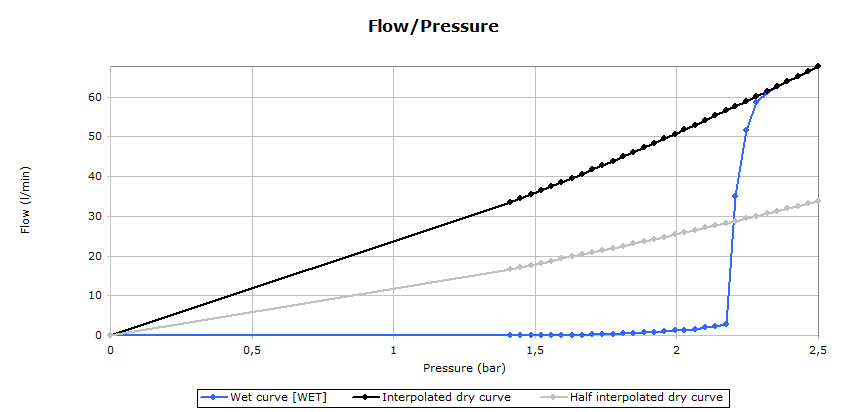
\includegraphics[width=\textwidth, height=6cm, keepaspectratio]{exemplocurvasporometer.png}
    \caption{Exemplo das curvas seca e molhada gerada pelo Porometer.}
    \label{fig:exemplocurvas}
\end{figure}


A análise com o goniômetro utiliza o método da séssil, onde uma gota de água deionizada é colocada sobre a superfície da membrana e fotografado por um sistema de alta resolução, permitindo medir o ângulo de contato entre a superfície da membrana e a gota. Foram realizadas três medições para cada membrana. A análise com o microcópio digital permitiu visualizar a estrutura dos suportes empregados nas membranas. A figura \ref{fig:hirox} apresenta os equipamentos utilizados.

 \begin{figure}[H]
    \centering
    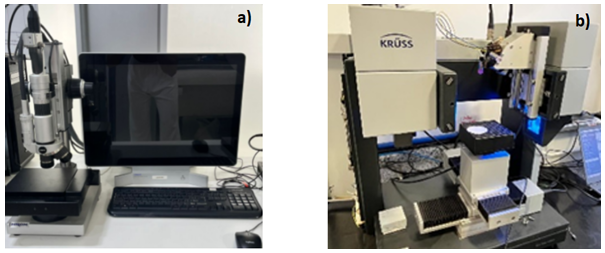
\includegraphics[width=\textwidth, height=12cm, keepaspectratio]{hirox.png}
    \caption{Microscópio digital a) e goniômetro de ângulo de contato b) utilizados no processo de caracterização das membranas.}
    \label{fig:hirox}
\end{figure}

\section{Características da água de produção}

A água de produção utilizada nos experimentos pertence a um campo de extração localizado no Brasil. A composição da água de produção foi definida através de duas amostras, retiradas em dias distintos. A análise da composição da água foi realizada pela empresa que forneceu as amostras.

Uma vez que os compostos orgânicos apresentam alta volatilidade em temperatura ambiente, adicionou-se a concentração dos mesmos à água de produção, em via de garantir a presença destes contaminantes.

\begin{table}[H]
\centering
\caption{Características analíticas de referência da água de produção utilizada nos experimentos.}
\label{tab:produced_water}

\begin{tabular}{lccc}
\hline
\textbf{Parâmetro} & \textbf{Unidade} & \textbf{18/Jan/2024} & \textbf{10/Jul/2024} \\ \hline

\multicolumn{4}{l}{\textbf{Análises físico-químicas}} \\

pH (25~$^\circ$C) & -- & 6,18 & 6,56 \\
Temperatura & $^\circ$C & 24,80 & 25,00 \\
Nitrogênio amoniacal & $mgL^{-1}$ & 36,00 & 81,00 \\
Óleos e graxas & $mgL^{-1}$ & $<$5,00 & $<$5,00 \\
Carbono orgânico total (COT) & $mgL^{-1}$ & 597,20 & 0,60 \\
Salinidade & \% & 23,50 & 23,50 \\

\hline

\multicolumn{4}{l}{\textbf{Metais}} \\

Bário & $mgL^{-1}$ & 9,62 & 14,50 \\
Ferro & $mgL^{-1}$ & 0,23 & 0,67 \\
Manganês & $mgL^{-1}$ & 0,13 & 0,14 \\
Zinco & $mgL^{-1}$ & $<$0,05 & 0,14 \\

\hline

\multicolumn{4}{l}{\textbf{Compostos orgânicos BTEX}} \\

Benzeno & $\mu gL^{-1}$ & 5523,11 & 2203,33 \\
Tolueno & $\mu gL^{-1}$ & 4055,78 & 1918,89 \\
Etilbenzeno & $\mu gL^{-1}$ & 471,78 & 177,06 \\
Xilenos totais & $\mu gL^{-1}$ & 2727,11 & 1096,00 \\

\hline

\multicolumn{4}{l}{\textbf{Hidrocarbonetos aromáticos policíclicos (PAHs)}} \\

Fenantreno & $\mu gL^{-1}$ & 6,34 & 1,53 \\
Fluoreno & $\mu gL^{-1}$ & 1,65 & 0,49 \\
Naftaleno & $\mu gL^{-1}$ & 84,27 & 1,34 \\

\hline
\end{tabular}
\end{table}
\newpage

\section{Análise de dados}

Calculou-se o LEP com base nos resultados obtidos durante a caracterização das membranas através da equação de Young-Laplace \ref{eq:LEP}:

\begin{equation}
    LEP = -\frac{2 \cdot B \cdot \gamma_L \cos\theta}{r_{\max}},
    \label{eq:LEP}
\end{equation}

onde $\gamma_L$ é a tensão superficial do líquido, $\theta$ é o ângulo de contato entre o líquido e a superfície da membrana, $r_{\max}$ é o maior raio de poro da membrana e $B$ o fator de forma atribuído ao poro. No presente estudo o fator de forma foi considerado como 1, de modo a considerar o poro como um cilindro ideal. 

Os parâmetros de performance do equipamento serão calculados em função da transferência de calor no lado quente e frio do módulo, além do fluxo de permeado produzido. A taxa de transferência de calor no lado quente e frio foram calculadas através das equações \ref{eq:Qcold} e \ref{eq:Qhot}, respectivamente: 

\begin{equation}
    Q_{\mathrm{cold}} = \dot{m}_c \, c_{p,c} \left( T_{c,out} - T_{c,in} \right),
    \label{eq:Qcold}
\end{equation}

\begin{equation}
    Q_{\mathrm{hot,sens}} = \dot{m}_h \, c_{p,h} \left( T_{h,in} - T_{h,out} \right),
    \label{eq:Qhot}
\end{equation}

onde $\dot m$ é a vazão mássica, $c_p$ é o calor específico, os subscritos $h, c, in, out$ representam o lado quente, frio, entrada e saída, respectivamente. As propiedades termofísicas da água de produção, como densidade e calor específico, serão avaliadas em função da salinidade através das correlações propostas por \cite{Millero1980}.

Uma estimativa da quantidade de calor fornecida pelo módulo para a evaporação do permeado será calculada através da equação \ref{eq:Qvap}, onde $T_{ref}$ é a temperatura de referência, calculada considerando as temperaturas dos escoamentos frio e quente através da equação \ref{eq:Tref}.

\begin{equation}
    Q_{\mathrm{vap}} = \dot{m}_p \, h_{lv}(T_{\mathrm{ref}}),
    \label{eq:Qvap}
\end{equation}

\begin{equation}
    T_{\mathrm{ref}} =
\frac{
\left( T_{h,in} + T_{h,out} \right)/2
+
\left( T_{c,in} + T_{c,out} \right)/2
}{2}
    \label{eq:Tref}
\end{equation}

O fluxo de permeado será obtido através de um sensor de pressão instalado no fundo do reservatório de permeado, obtido através da equação \ref{eq:fluxo}, onde $A_B$ é a área da base do reservatório de permeado, $A_m$ é a área efetiva da membrana, g é a gravidade, $\Delta P / \Delta t$ é a taxa de variação da pressão ao longo do tempo, obtendo-se o resultado em $kgm^{-2}h^{-1}$.

\begin{equation}
J = \frac{A_B}{g \, A_m}
\left( \frac{\Delta P}{\Delta t} \right)
3600
    \label{eq:fluxo}
\end{equation}

O índice de rejeição instantânea de íons, IJR, será obtido através da equação \ref{eq:IJR}, onde $k_p$ e $k_f$ representam as condutividades do permeado e da água de produção, respectivamente. 

\begin{equation}
IJR =
\left(
1 - \frac{\kappa_p}{\kappa_f}
\right)
\times 100
    \label{eq:IJR}
\end{equation}

O fator de desempenho térmico, GOR, será calculado através da equação \ref{eq:GOR} como a razão entre o calor latente associado ao fluxo de permeado pelo calor sensível fornecido ao módulo.

\begin{equation}
GOR = \frac{\dot{m}_p \, h_{lv}}{Q_{\mathrm{hot}}}
    \label{eq:GOR}
\end{equation}

Por fim, o consumo de energia térmica específica será calculada através da equação \ref{eq:SEC}, como a razão entre a energia térmica fornecida pelo volume de permeado produzido, $V_p$.

\begin{equation}
SEC_{\mathrm{th}} =
\frac{Q_{\mathrm{hot}}}{V_p}
\quad
\left[\mathrm{J/m^3}\right]
    \label{eq:SEC}
\end{equation}

As incertezas associadas as variáveis primárias de medição, como temperatura, vazão, pressão e condutividade serão propagadas através aos indicadores de performance através da lei de propagação de variáveis.